\chapter{El primer rayo de Sol -- I}
\label{cap:el-primer-rayo-de-sol-i}

\lettrine[ante=\raisebox{-1.5ex}{\Large ---},lines=2]{V}{amos a ver}
ahora cómo escribir uno de los paralelepípedos con los que cortaremos
el cuerpo de nuestro reloj; ¿te acordás?  ---pre\-gun\-tó Antonia al
día siguiente. Cecilia, por su parte, no sólo lo recordaba
perfectamente sino que estaba ansiosa por llevarlo a cabo.

\vspace{1em}

\begin{figure}[ht]
  \centering
  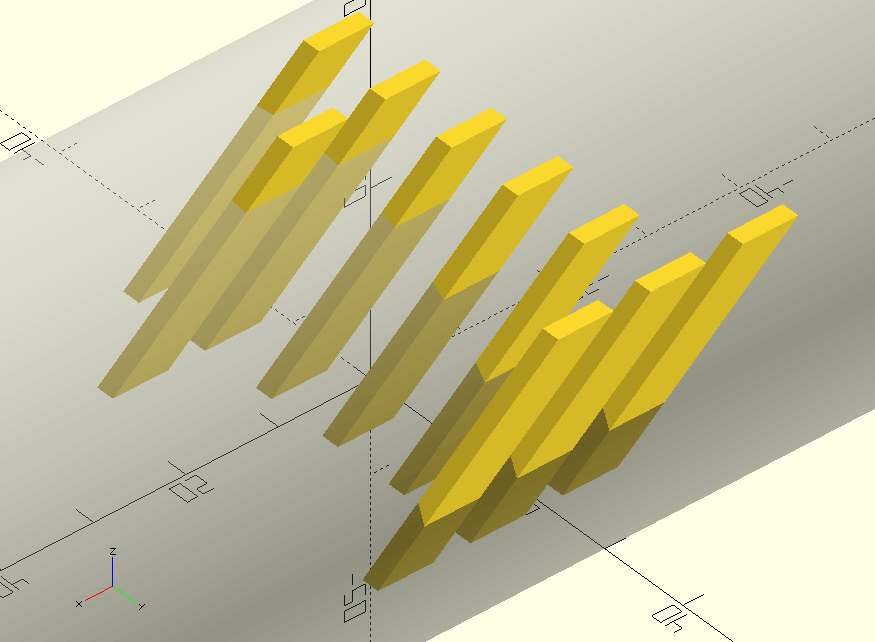
\includegraphics[width=.49\textwidth]{imagenes/digito-soslayo}\hfill
  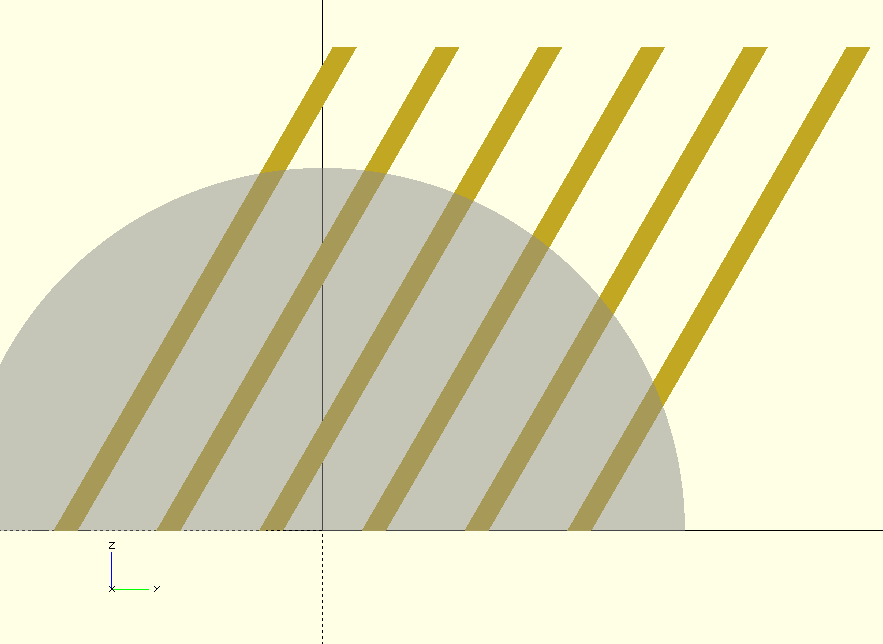
\includegraphics[width=.49\textwidth]{imagenes/digito-perfil} 
  \caption{Antonia materializa los rayos de Sol como paralelepípedos
    que cortan el cuerpo del reloj para indicar así, bajo determinado
    ángulo, un dígito preciso: en este caso, el \texttt{1}.}
  \label{fig:digitos-soslayo-perfil}
\end{figure}


\guillemotright Supongo que habrá otras maneras de resolverlo
---An\-to\-nia se encogió de hombros---; pero a mí me resultó natural
pensarlo así: en primer lugar, llamé `pixeles' a cada una de las caras
que forman un dígito. ¡Qué se yo! Necesitaba un nombre, y me pareció
tan bueno como cualquier otro, además de que me evocaba la idea de
aquellos `puntos' que conforman una imagen digital.

A Cecilia no le pareció que tal decisión mereciera objeción alguna, ni
tampoco una defensa encendida.

\begin{figure}[ht]
  \centering
  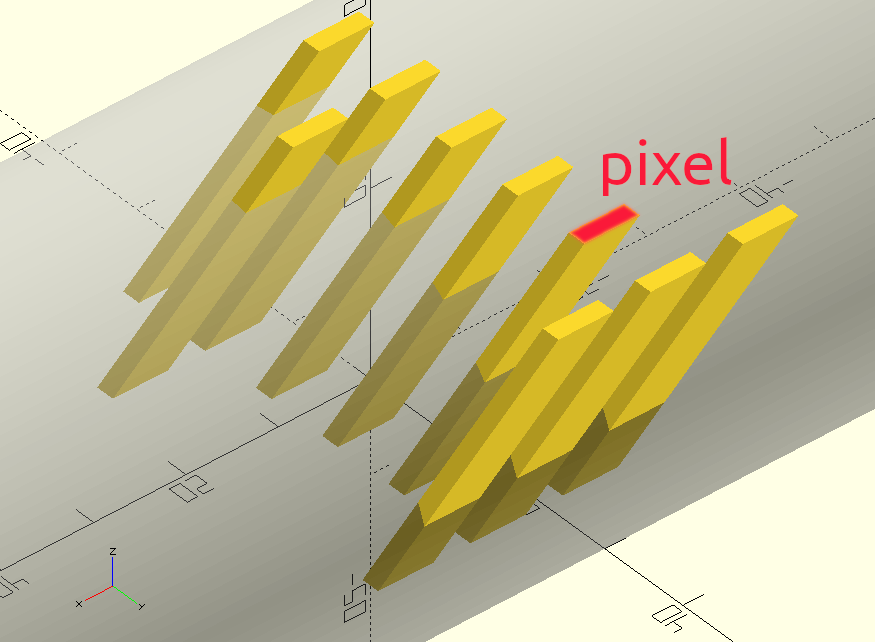
\includegraphics[width=.5\textwidth]{imagenes/digito-soslayo-pixel}
  \caption{Antonia decide llamar ``pixeles'' a las caras superiores de
    los rayos de Sol que cortan el cuerpo del reloj.}
  \label{fig:digito-soslayo-pixel}
\end{figure}

---Cada pixel tendrá un ancho y un alto, que deberían poder ser
elegidos por el usuario ---afirmó Antonia dirigiendo la mirada de su
amiga a la figura \ref{fig:pixel-alto-ancho}.


\begin{figure}[ht]
  \centering
  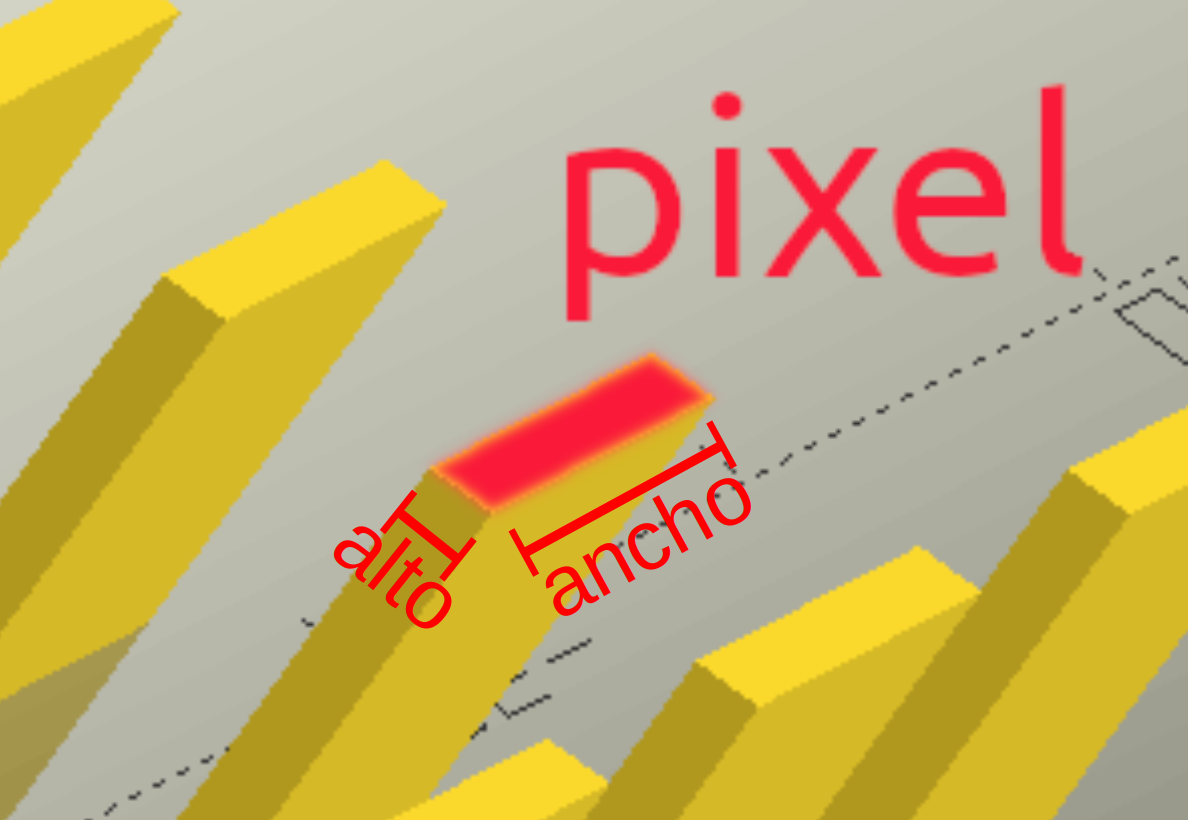
\includegraphics[width=.5\textwidth]{imagenes/pixel-alto-ancho}  
  \caption{Los pixeles tendrán sus debidos ancho y alto.}
  \label{fig:pixel-alto-ancho}
\end{figure}


\guillemotright Ahora, me imaginé cada pixel extrudido a partir de un
polígono con uno de los perfiles de la figura
\ref{fig:digito-perfil-extrudido}.

\begin{figure}[ht]
  \centering
  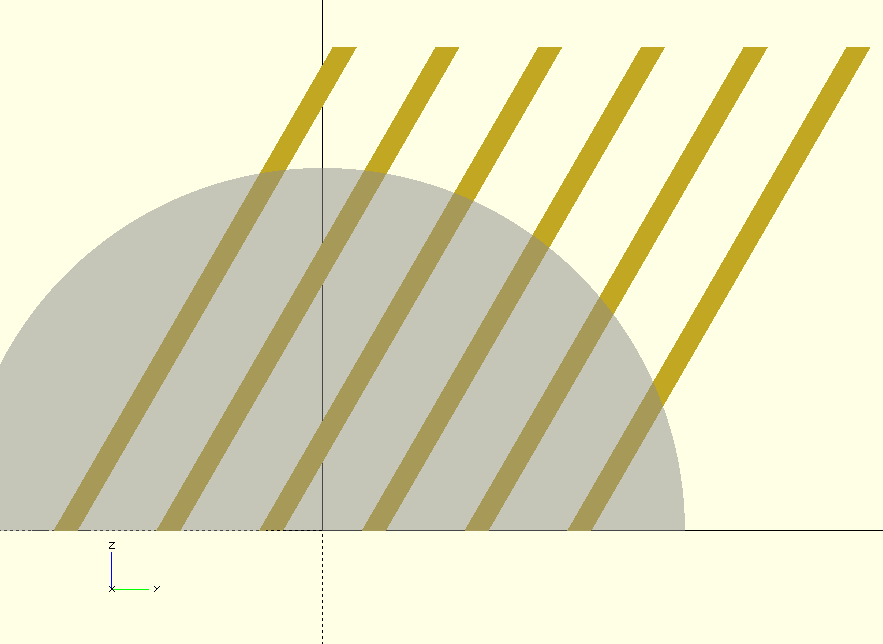
\includegraphics[width=.49\textwidth]{imagenes/digito-perfil}\hfill
  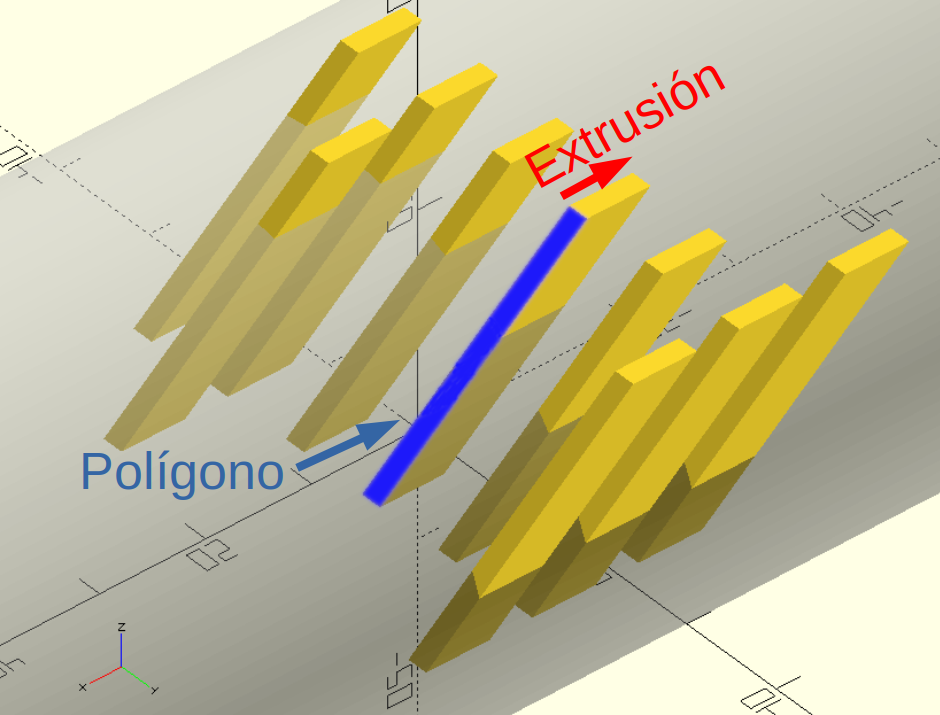
\includegraphics[width=.49\textwidth]{imagenes/digito-extrudido}
  \caption{Antonia pretende erigir los rayos de Sol extruyendo
    polígonos, uno de los cuales destacó en azul.}
  \label{fig:digito-perfil-extrudido}
\end{figure}

\guillemotright Y ahora, Cecilia ---advirtió Antonia---, preparate
porque se viene una andanada de pura geometría. Agarrate fuerte.

Cecilia quiso recordarle que estaba hablando con una doctora en
ciencias; pero por un lado le pareció un poco pedante, y por otro no
estaba tan segura de recordar cómo manejarse entre los vericuetos
euclídeos en los que Antonia estaba a punto, sin duda, de aventurarse.

---Supongamos que ya calculamos la dirección en la que debe
encontrarse el Sol al momento en que queremos que, debajo del reloj,
aparezca el dígito deseado. Esa dirección estará determinada por un
ángulo, que ya veremos cómo calcular gracias a nuestros fantásticos
conocimientos astronómicos: llamémoslo $\alpha$ ---dijo Antonia
señalando la figura \ref{fig:poligono-alfa}.

\begin{figure}[ht]
  \centering
  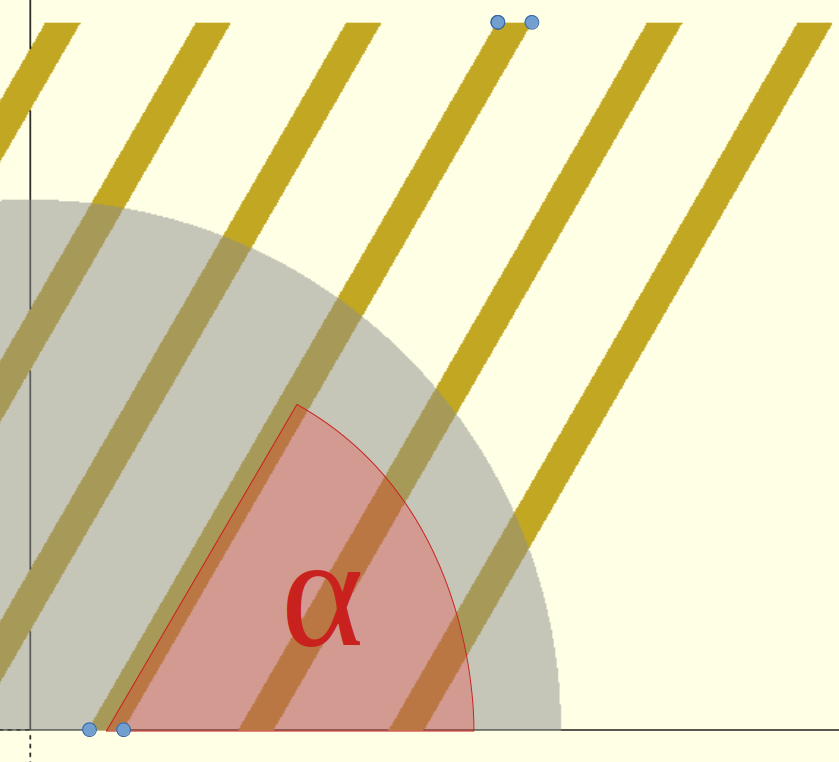
\includegraphics[width=.4\textwidth]{imagenes/poligono-pixel}
  \caption{La inclinación de cada rayo estará determinada por la
    altura del Sol en cada momento, señalada con el ángulo $\alpha$.}
  \label{fig:poligono-alfa}
\end{figure}


\guillemotright Pues bien ---Antonia parecía finalmente acercarse,
tras algunos rodeos, a algún tipo de definición---; nuestro objetivo
ahora es encontrar las coordenadas de los vértices del polígono que
queremos luego extrudir: los destaqué con circulitos azul pálido en la
misma figura: ¿los ves?

Cecilia los veía, pero no cómo calcularlos. <<¿Trigonometría?>>
---pensó.

---Hay que usar trigonometría ---soltó Antonia como si hubiera hecho
una revelación---.  No es tan difícil. Primero fijemos el punto origen
del polígono; podría ser cualquiera, y a mí me resultó natural elegir
el que señalé en la figura \ref{fig:poligono-origen}.

\begin{figure}[ht]
  \centering
  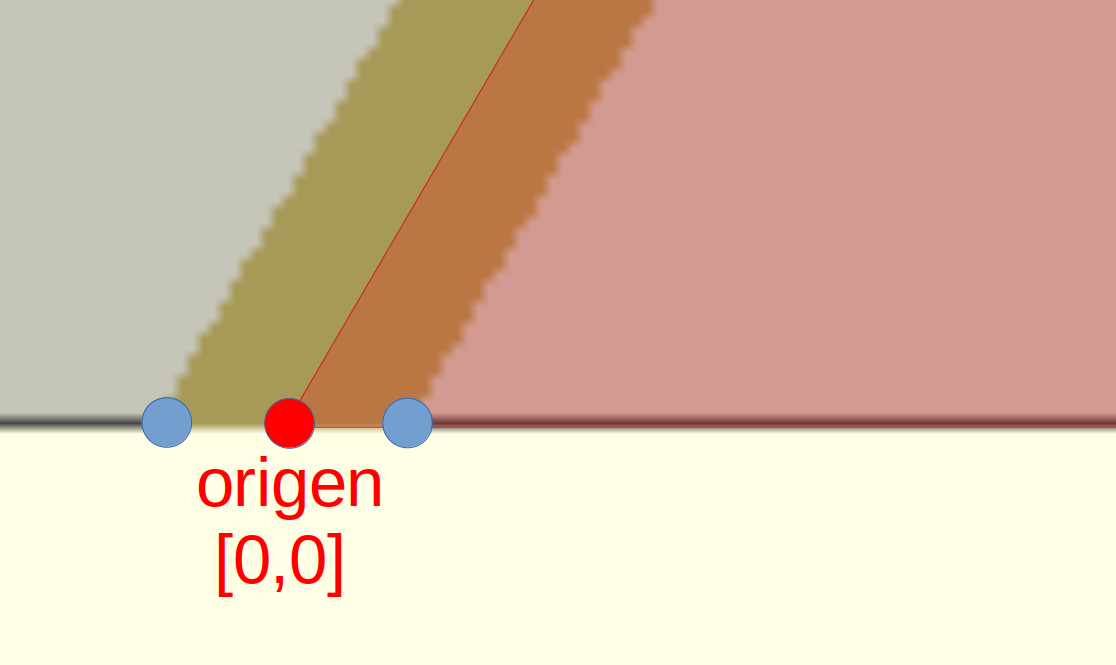
\includegraphics[width=.45\textwidth]{imagenes/poligono-origen}
  \caption{Antonia elige como origen de cada polígono el punto medio
    de su arista inferior.}
  \label{fig:poligono-origen}
\end{figure}


\guillemotright Sus coordenadas, por definición, son \texttt{[0,0]}: 0
en \coord{X} y 0 en \coord{Y}. Así, las coordenadas de los dos puntos
de la base de nuestro polígono creo que son inmediatas ---aseguró,
señalando la figura \ref{fig:poligono-puntos-base}.


\begin{figure}[ht]
  \centering
  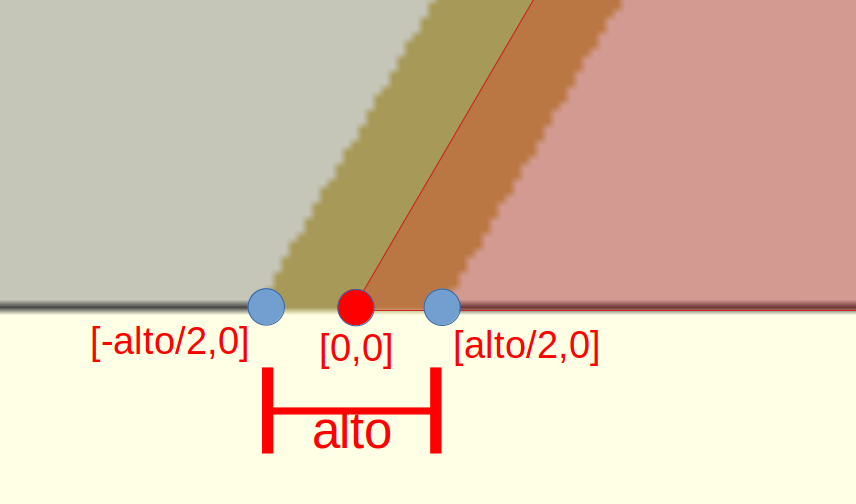
\includegraphics[width=.53\textwidth]{imagenes/poligono-puntos-base}\hfill
  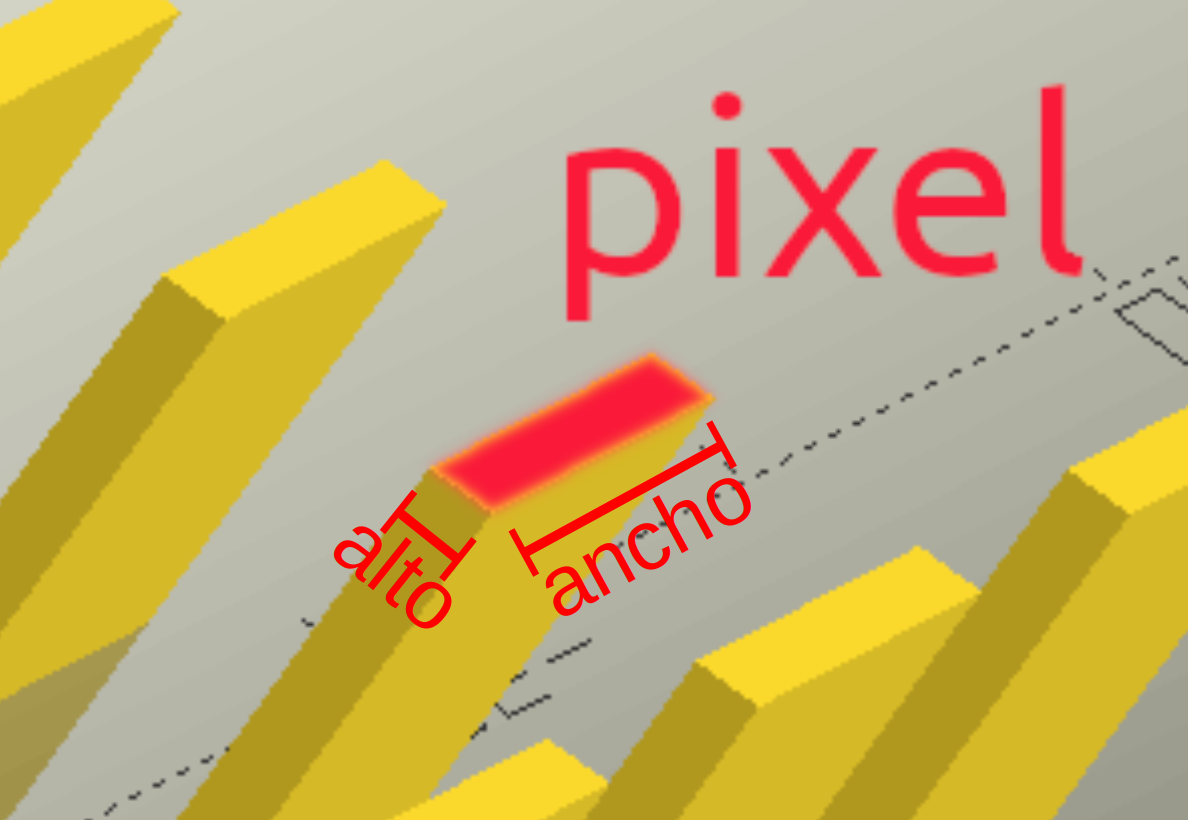
\includegraphics[width=.45\textwidth]{imagenes/pixel-alto-ancho}  
  \caption{Antonia marca las coordenadas de los extremos inferiores
    del polígono buscado.}
  \label{fig:poligono-puntos-base}
\end{figure}

Cecilia, al principio, se confundió un poco; pero recordó que el
\texttt{ancho} del polígono se correspondía con el \texttt{alto} del
píxel final. Comprendió que, con respecto al origen elegido, ambos
puntos tenían la misma coordenada \coord{Y} (y, por lo tanto igual a
0), y diferían de él en una distancia igual a $\frac{\text{alto}}{2}$
en \coord{X}, una con signo positivo y otra negativo.

---Muy bien ---dijo Antonia, quizá no muy satisfecha con su propia
explicación---; ahora veamos los dos vértices superiores. A mí, para
fijar ideas, me resultó útil pensar en un punto auxiliar, ubicado
justo en medio de dichos vértices, tal como se aprecia en la figura
\ref{fig:poligono-punto-auxiliar}.
  

\begin{figure}[ht]
  \centering
  
\includegraphics[width=.7\textwidth]{imagenes/poligono-punto-auxiliar}  
  \caption{Antonia busca las coordenadas de los extremos superiores
    del polígono mediante un punto auxiliar, ubicado en medio de
    ambos.}
  \label{fig:poligono-punto-auxiliar}
\end{figure}


\guillemotright Podemos referirnos a la posición de ese punto auxiliar
mediante dos valores: $D$ y $H$. El primero será su distancia
horizontal con respecto al origen; en otras palabras, su coordenada
\coord{X}. $H$, análogamente, será su coordenada \coord{Y}
---ex\-pli\-có Antonia, señalando la figura
\ref{fig:poligono-tangente}.

\begin{figure}[ht]
  \centering
  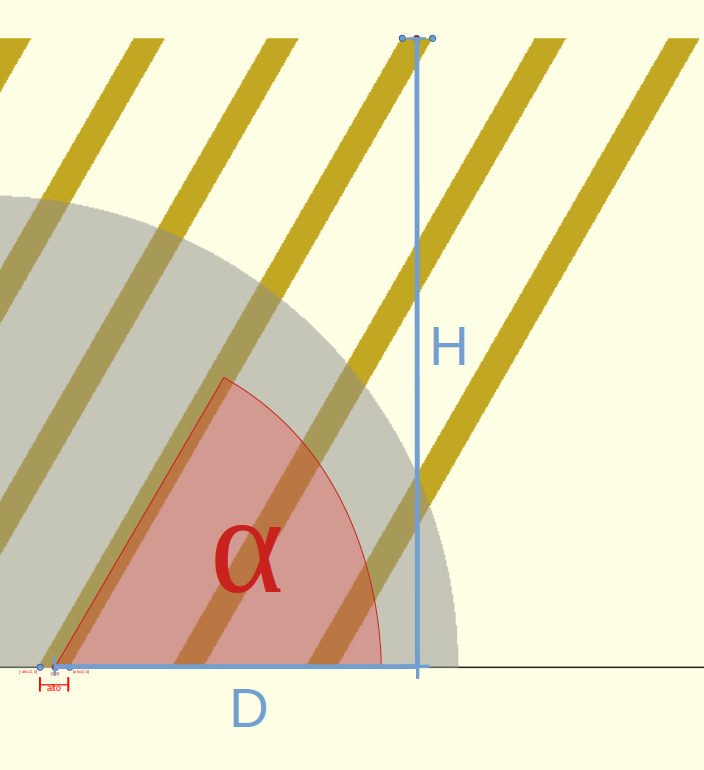
\includegraphics[width=.4\textwidth]{imagenes/poligono-tangente}
  \caption{Antonia señala las coordenadas del nuevo punto auxiliar.}
  \label{fig:poligono-tangente}
\end{figure}


---¿Así que las coordenadas de tu nuevo punto auxiliar serán
\texttt{[D,H]}? ---preguntó Cecilia, no tanto para confirmar que
entendía como para animar a su amiga a continuar.

---¡Exacto! ---exclamó Antonia con el súbito entusiasmo que se
apoderaba de ella cuando sucumbía a la ilusión de ser
com\-pren\-di\-da---.  Ahora bien, habíamos quedado en que el valor de
$\alpha$ era conocido por nosotras\footnote{Espero que le dediquen un
  capítulo a esta delicada cuestión. (Nota del
  Editor)}$^,$\footnote{¡No te preocupes!  ¡Lo haremos! ¡Qué
  ansioso..! (Nota de Antonia y Cecilia)}; de esa manera, la
trigonometría nos promete que hay una firme relación entre $\alpha$,
$D$ y $H$, gracias a la función \texttt{tangente}:

\begin{equation}
  \tan \alpha = \frac{H}{D}\label{eq:tangente}
\end{equation}

Cecilia recordaba claramente esa relación; supuso que \openscad{}
sabría cómo calcularla.

---\openscad{}, por supuesto, cuenta entre sus funciones elementales
la \texttt{tangente} ---Antonia volvió a leer la mente de Cecilia,
quien ya estaba comenzando a preocuparse por esa clarividencia tan
oportuna. Por momentos le hacía pensar que su vida no era real, sino
que formaba parte de un cuento, o tal vez un manual mal escrito.

---Hasta ahora, todo muy bonito, Antonia ---interrumpió Cecilia,
visiblemente incómoda---; comprendo que $\alpha$ lo podemos calcular
astronómicamente, pero: ¿Qué onda $D$ y $H$? Una única ecuación no nos
permite calcular dos valores simultáneamente ---preguntó, con tono
casi acusador.

Antonia asintió suavemente con la cabeza, mientras fruncía los
labios:

---Tenés razón; y acá tuve que tomar una decisión más. ¡Ay, Cecilia!
---suspiró, reclinándose contra la silla---.  ¡La programación, como
la vida, exige constantemente de nosotras la toma de decisiones..!
---Antonia se detuvo un momento, como buscando un recuerdo---. A ver
si puedo mostrarte la manera en que lo pensé...

Tras escribir unos instantes, durante los cuales creó las imágenes de
la figura \ref{fig:rayos-10-30-60-80}, Antonia continuó:



\begin{figure}[ht]
  \centering
  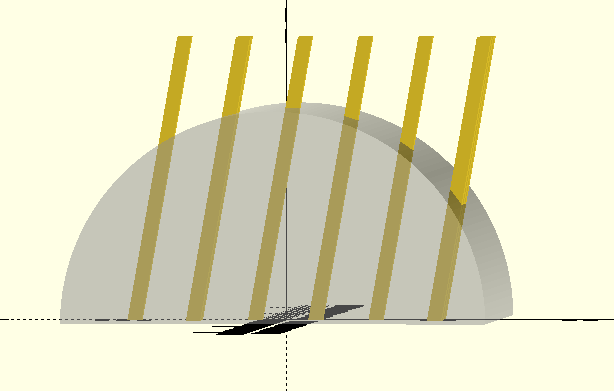
\includegraphics[width=.49\textwidth]{imagenes/rayos-10}\hfill
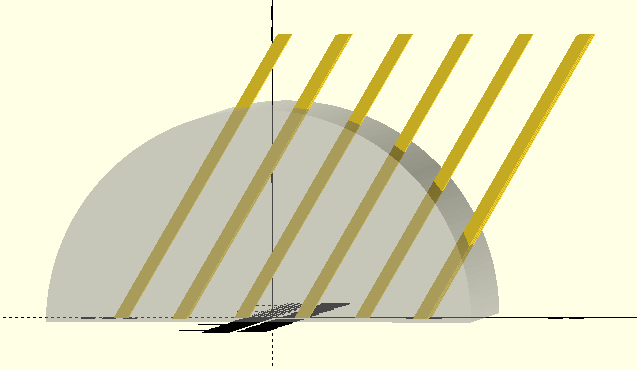
\includegraphics[width=.49\textwidth]{imagenes/rayos-30}
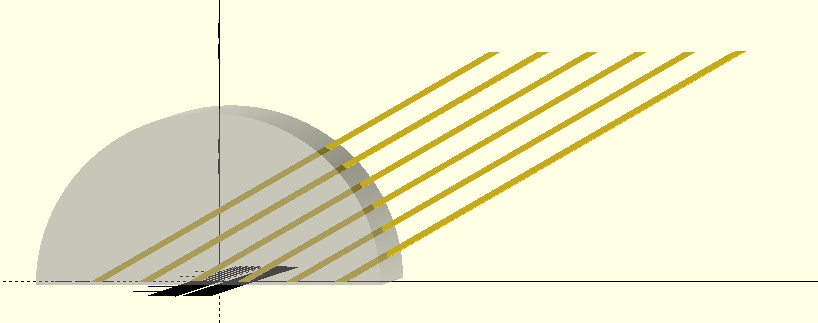
\includegraphics[width=.9\textwidth]{imagenes/rayos-60}
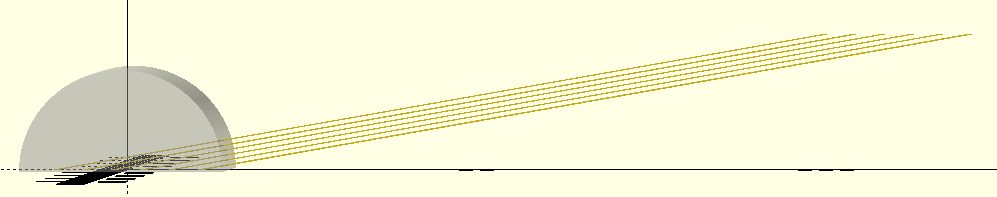
\includegraphics[width=1\textwidth]{imagenes/rayos-80}
\caption{Antonia despliega para Cecilia distintos grupos de rayos con
  diferentes ángulos $\alpha$, a fin de que descubra la relación que
  guarda el mismo con $D$ y $H$ en todos los casos.}
\label{fig:rayos-10-30-60-80}
\end{figure}

---Aquí dispuse el mismo dígito, formado por cierto número de pixeles,
con distintos ángulos $\alpha$, correspondientes a diferentes
posiciones del Sol ---Antonia dirigió su mirada a Cecilia, y en sus
ojos había una luz que parecía una súplica---. ¿Notás algún patrón que
se repita en todos los casos..?

  Cecilia sintió súbitamente sobre sus hombros una grave
  responsabilidad: no tanto por salvaguardar su reputación de
  ``inteligente'', sino para que Antonia no sintiera que su
  explicación la conducía a una confusión irremontable.  Como tantos
  otros alumnos antes y después que ella, sintió la piadosa obligación
  de justificar a su maestra. Con la mirada y la mente concentradas en
  el monitor, contempló los cuatro casos que Antonia le
  ofrecía.% Trató
  % de evitar la confusión de las distintas escalas, que le mostraban
  % los primeros más grandes que los últimos.

  <<¿Qué tendrán en común estos dichosos ejemplos...?>> \mbox{---pen}\-só, al
  borde del malhumor y de rendirse. Pero de pronto y sin saber de
  dónde, la epifanía ocurrió:

  ---¿Puede ser que todos los rayos tengan la misma altura? ¿Es decir,
  que compartan el mismo $H$, en todos los casos y con cualquier
  ángulo? ---dijo.

  El suspiro de alivio de Antonia debió haberse oído hasta en la
  oficina de \director:

  ---Sí, Cecilia... sí ---Antonia estaba radiante---. El valor de $H$
  es convencional; es importante, eso sí, que sea mayor al radio del
  semicilindro, para que los rayos puedan cortarlo siempre. Es cierto
  ---reconoció--- que eso hará que los mismos resulten muy largos para
  ángulos muy bajos; pero, como ya conversamos alguna vez, rayos muy
  dilatados no ocupan más sitio en la memoria de la computadora que
  otros más cortos.

  A Cecilia empezó a parecerle una solución muy astuta:

  ---Así que elegimos un $H$ cualquiera y fijo, más grande que el
  radio del semicilindro, y con $\alpha$ y la ecuación
  \ref{eq:tangente} calculamos $D$ ---re\-su\-mió, quizá para
  comprobar que había entendido.

  Antonia aplaudió lentamente, mientras asentía con la cabeza. Cecilia
  no supo discenir para quién era la felicitación.

  ---Con lo visto, las coordenadas de los vértices superiores del
  polígono deberían resultar fáciles de determinar ---confió Antonia.


  \begin{figure}[ht]
    \centering
    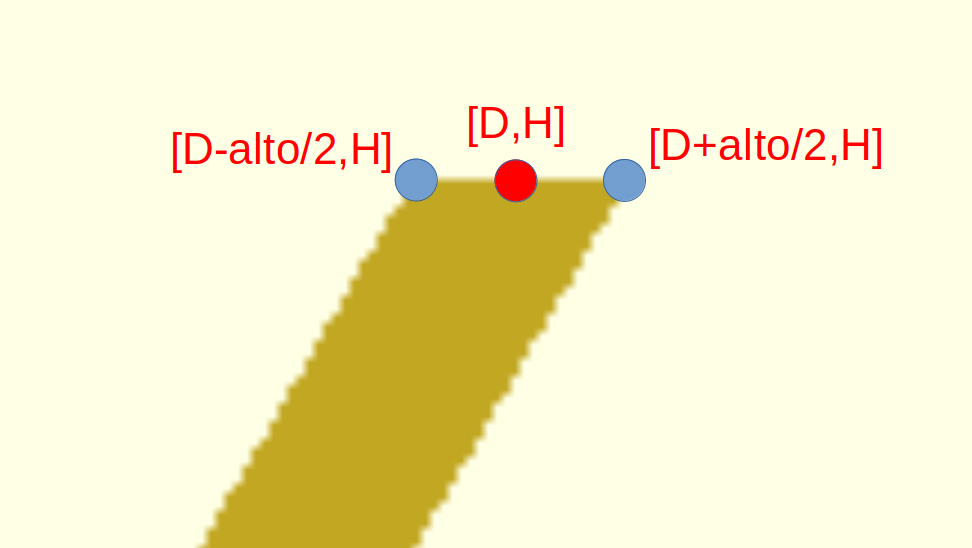
\includegraphics[width=.65\textwidth]{imagenes/poligono-tapa}    
    \caption{Antonia explicita las coordenadas de los vértices
      superiores.}
    \label{fig:poligono-tapa}
  \end{figure}


  \guillemotright Así que nuestro rayo de Sol debería comenzar con un
  polígono cuyos vértices, referidos a un cierto origen de
  coordenadas, sean \texttt{[-alto/2,0], [D-alto/2,H], [D+alto/2,H],
    [alto/2,0]}.


    \begin{lstlisting}
alto_pixel = 2;
ancho_pixel = 6;
radio_semicilindro = 30;
H = radio_semicilindro+10;

module rayo_de_sol(alfa){
  D=H/tan(alfa);
  vertices=[[-alto_pixel/2,0],
            [D-alto_pixel/2,H],
            [D+alto_pixel/2,H],
            [alto_pixel/2,0]];
  polygon(vertices);
}
 
rayo_de_sol(alfa=60);
\end{lstlisting}
%   \end{center}
% \begin{center}

\begin{figure}[ht]
  \centering
  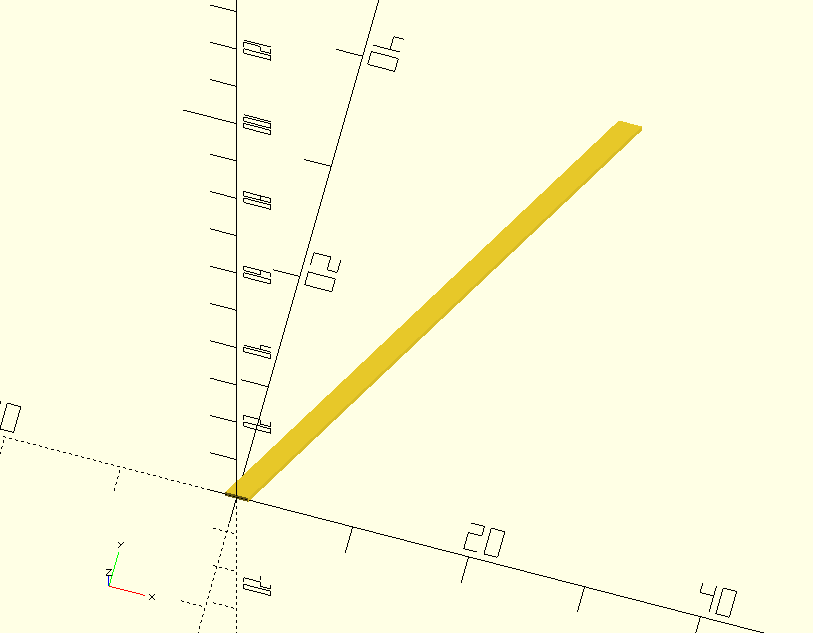
\includegraphics[width=.65\textwidth]{imagenes/rayo-de-sol-1}
  \caption{Antonia, finalmente, está en condiciones de escribir el
    código del polígono de un rayo de Sol.}
  \label{fig:rayo-de-sol-1}
\end{figure}


Cecilia no pudo disimular su emoción: ¡Por fin algo de texto!  Sintió
que nada le confirmaría mejor que iban por un buen camino que el
funcionamiento cabal de un programa que reflejara fielmente las ideas
que elaboraban juntas.

---Por supuesto ---aclaró Antonia---, el rayo no está terminado: por
ahora es sólo un polígono recostado en el plano \coord{XY}. Debemos
convertirlo en un genuino objeto 3D mediante una extrusión lineal, y
luego pararlo mediante una rotación.

---Sí, Antonia, entiendo; ¿pero no podemos dejarlo para el capítulo
siguiente? Por éste creo que ya vimos mucho \mbox{---su}\-pli\-có Cecilia, quien
estuvo a punto de utilizar la palabra ``demasiado'' en lugar del más
diplomático ``mucho''.
  

%%% Local Variables:
%%% mode: latex
%%% TeX-master: "../libro"
%%% End:
